\documentclass{beamer} 
\usepackage{amsmath,amsthm}
\usepackage{graphicx,microtype,parskip}
\usepackage{caption,subcaption,multirow}
\usepackage{attrib}

\frenchspacing

\usetheme{default}
\usecolortheme{whale}

\setbeamertemplate{navigation symbols}{}

\setbeamercolor{title}{fg=blue,bg=white}

\setbeamercolor{block title}{fg=white,bg=gray}
\setbeamercolor{block body}{fg=black,bg=lightgray}

\setbeamercolor{block title alerted}{fg=white,bg=darkgray}
\setbeamercolor{block body alerted}{fg=black,bg=lightgray}

%\AtBeginSection[]
%{
%  \begin{frame}
%    \tableofcontents[currentsection]
%  \end{frame}
%}

\title{How do biological traits affect brachiopod taxonomic survival?}
\subtitle{A hierarchical Bayesian approach}
\author{Peter D Smits}
\institute{Committee on Evolutionary Biology, University of Chicago}
\titlegraphic{
  \includegraphics[width=2.75cm,height=2.75cm,keepaspectratio=true]{figure/paleodb}
  \hspace*{0.35\paperwidth}
  \includegraphics[width=2cm,height=2cm,keepaspectratio=true]{figure/chicago}
}
\date{}

\begin{document}

\begin{frame}
  \maketitle
\end{frame}

\begin{frame}
  \begin{alertblock}{Observation}
    At K/Pg mass extinction, biological traits (except geographic range) have no effect on taxonomic survival.
    
    \attrib{\footnotesize{Jablonski, 1986, \em{Science}}}
  \end{alertblock}
\end{frame}

\begin{frame}
  \frametitle{Macroevolutionary process hypotheses}
  \begin{center}
    \begin{columns}
      \begin{column}{0.45\textwidth}
        As extinction risk increases, the effect of geographic range increases.
      \end{column}
      \begin{column}{0.05\textwidth}
        \textbf{-----}
      \end{column}
      \begin{column}{0.45\textwidth}
        As extinction risk increases, the effects of other traits decrease.
      \end{column}
    \end{columns}
  \end{center}
\end{frame}

\begin{frame}
  \frametitle{Relationship between range size and extinction risk}
  \begin{center}
    \includegraphics[width = \textwidth,height = 0.8\textheight,keepaspectratio = true]{figure/harnik_rarity}
  \end{center}

  \attrib{\footnotesize{Harnik and Simpson 2013 \textit{Proc B}}}
\end{frame}

\begin{frame}
  \frametitle{Survival of the unspecialized}
  \begin{quote}
    When related phyla die out \dots more specialized phyla tend to become extinct before less specialized. This phenomenon is also far from universal, but it is so common that it does deserve recognition as a rule or principle in evolutionary studies: \textbf{the rule of the survival of the relatively unspecialized.}

    \attrib{\footnotesize{Simpson, 1944, \em{Tempo and Mode of Evolution}, p. 143}}
  \end{quote}
\end{frame}

\begin{frame}
  \frametitle{Hypotheses of effect of environmental preference}
  \includegraphics[width = \textwidth,height = 0.8\textheight,keepaspectratio = true]{figure/miller_foote}

  \attrib{\footnotesize{Miller and Foote 2009 \textit{Science}}}
\end{frame}

\begin{frame}
  \frametitle{Hypotheses of effect of environmental breadth}

  \begin{center}
    \includegraphics[width = \textwidth,height = 0.8\textheight,keepaspectratio = true]{figure/selection_breadth}
  \end{center}
\end{frame}

\begin{frame}
  \frametitle{Hierarchical bayesian model}
  \begin{center}
    \includegraphics[width = \textwidth,height = 0.8\textheight,keepaspectratio = true]{figure/han_bayes}
  \end{center}
\end{frame}

\begin{frame}
  \frametitle{Hierarchical survival model}
  \begin{center}
    \includegraphics[width = \textwidth,height = 0.8\textheight,keepaspectratio = true]{figure/simple_model}
  \end{center}
\end{frame}

\begin{frame}
  \frametitle{Paleozoic brachiopods}
  \begin{center}
    \includegraphics[width = \textwidth,height = 0.8\textheight,keepaspectratio = true]{figure/permian_brac}
  \end{center}
\end{frame}

\begin{frame}
  \frametitle{Posterior predictive distribution of S(t)}

  \begin{center}
    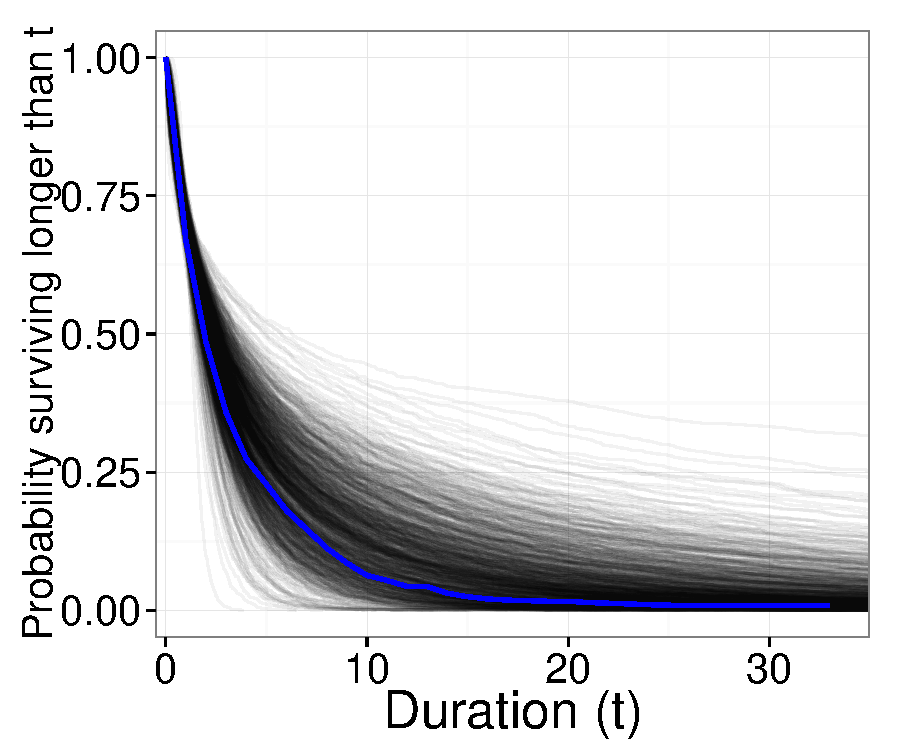
\includegraphics[width = \textwidth,height = 0.8\textheight,keepaspectratio = true]{figure/survival_curves}
  \end{center}
\end{frame}

\begin{frame}
  \frametitle{Change in trait effects between cohorts}

  \begin{center}
    \includegraphics[width = \textwidth,height = 0.8\textheight,keepaspectratio = true]{figure/cohort_series}
  \end{center}
\end{frame}

\begin{frame}
  \frametitle{Overall effect of environmental preference}

  \includegraphics[width = \textwidth,height = 0.8\textheight,keepaspectratio = true]{figure/environ_quad}
\end{frame}

\begin{frame}
  \frametitle{Change in effect of environment between cohorts}

  \includegraphics[width = \textwidth,height = \textheight,keepaspectratio = true]{figure/cohort_quads_short}
\end{frame}

\begin{frame}
  \frametitle{Change in effect of environment between cohorts}

  \includegraphics[width = \textwidth,height = \textheight,keepaspectratio = true]{figure/cohort_quads}
\end{frame}

\begin{frame}
  \frametitle{Correlation of effects between cohorts}

  \begin{center}
    \includegraphics[width = \textwidth,height = 0.9\textheight,keepaspectratio = true]{figure/wei_cor_heatmap}
  \end{center}
\end{frame}

\begin{frame}
  \begin{block}{Effect summary}
    \begin{itemize}
      \item Effect of geographic range consistent with prior expectations.
      \item No effect of body size; environmental preference equal.
      \item Weak support for survival of unspecialized as generalization.
    \end{itemize}
  \end{block}
\end{frame}

\begin{frame}
  \begin{block}{Correlation of effects}
    \begin{itemize}
      \item Correlation between baseline extinction risk and effects of geographic range as well as environmental breadth.
      \item Correlation between effect of range and effect of environmental breadth.
        \begin{itemize}
          \item As effect of geographic range increases, decrease in selection on environmental breadth.
        \end{itemize}
    \end{itemize}
  \end{block}
\end{frame}

\begin{frame}
  \begin{alertblock}{Macroevolutionary process}
    \begin{itemize}
      \item As extinction risk increases, the effect of geographic range ``washes out'' the effects of other traits.
        \begin{itemize}
          \item Support for hypotheses presented in Jablonski 1986 Science, Raup 1994 PNAS.
        \end{itemize}
    \end{itemize}
  \end{alertblock}
\end{frame}

\begin{frame}
  \frametitle{Acknowledgements}
  \begin{columns}
    \begin{column}{0.5\textwidth}
      \begin{itemize}
        \item Advising
          \begin{itemize}
            \item Kenneth D. Angielczyk, Michael J. Foote, \\P. David Polly, \\Richard H. Ree, \\Graham Slater
          \end{itemize}
        \item Angielczyk Lab
          \begin{itemize}
            \item {\small{David Grossnickle, \\Dallas Krentzel, \\Jackie Lungmus}}
          \end{itemize}
        \item Foote lab
          \begin{itemize}
            \item {\small{Marites Villarosa Garcia, \\Nadia Pierrehumbert}}
          \end{itemize}
      \end{itemize}
    \end{column}
    \begin{column}{0.5\textwidth}
      \begin{itemize}
        \item {\footnotesize{Stewart Edie, \\Elizabeth Sander, \\Laura Southcott, \\Courtney Stepien}}
        \item {\footnotesize{David Bapst, \\Ben Frable, \\\textbf{Arnold Miller}, \\Peter Wagner}}
      \end{itemize}
      
      \vspace*{0.05\textheight}
      \begin{center}
        \includegraphics[height=0.2\textheight,width=\textwidth,keepaspectratio=true]{figure/paleodb}
      \end{center}
    \end{column}
  \end{columns}
\end{frame}

\end{document}
